\chapter{Simulações Computacionais}

Com o intuito de validar as expressões deduzidas analiticamente e atestar a eficácia do dimensionamento dos indutores, o circuito conversor \textit{Buck} simplificado foi implementado e submetido a ensaios transientes no simulador LTSpice \cite{ltspice}. Esta etapa computacional permite emular as condições de chaveamento de alta frequência e observar graficamente as parcelas de regime transitório e permanente da tensão na carga.

\section{Metodologia e Configuração do Ambiente de Simulação (LTSpice)}

Para assegurar uma correlação fidedigna entre o modelo matemático teórico e o ambiente simulado, exigiu-se uma configuração minuciosa dos parâmetros do software, mitigando as não-idealidades típicas de componentes comerciais. O \textit{setup} de simulação seguiu as seguintes diretrizes operacionais:

\subsection{Diretrizes SPICE e Modelagem de Semicondutores}
O roteiro laboratorial impõe o uso de modelos quase ideais para a chave e para o diodo de roda livre. Tais configurações foram aplicadas diretamente no esquemático através de comandos nativos do LTSpice (\textit{SPICE Directives}):
\begin{itemize}
	\item \textbf{Chave Controlada por Tensão (\texttt{sw}):}\\
	 Inseriu-se a diretriz \texttt{.model swi sw(Ron=1m Roff=10Meg Vt=0.98 Vh=0.01)}. Este comando define uma chave com resistência de condução quase nula ($1\text{ m}\Omega$), isolamento altíssimo na abertura ($10\text{ M}\Omega$) e um limiar de acionamento em $0,98\text{ V}$.
	\item \textbf{Diodo (\texttt{d}):}\\
	 Inseriu-se a diretriz \texttt{.model di d(Ron=1m Roff=10Meg Vfwd=0 Vrev=1k)}.\\
	 Com isso, elimina-se a queda de tensão de condução direta ($V_{fwd} = 0\text{ V}$), aproximando o componente do modelo teórico por partes utilizado na modelagem matemática.
\end{itemize}
Os componentes visuais no esquemático foram devidamente vinculados a estas diretrizes renomeando seus valores originais para \texttt{sw\_i} e \texttt{di}, respectivamente.

\subsection{Configuração do Sinal de Controle (Chaveamento)}
O acionamento da chave foi orquestrado por uma fonte de tensão de controle operando no modo \textbf{PULSE}. Como a chave \texttt{sw\_i} é ativada em $0,98\text{ V}$, o pulso foi configurado para transitar entre $V_{initial} = 0\text{ V}$ e $V_{on} = 1\text{ V}$. Para garantir flancos de subida e descida ideais, os parâmetros $T_{rise}$ e $T_{fall}$ foram ajustados para $1\text{ ns}$ (um nanossegundo). 
O ciclo de trabalho adotado foi estritamente de 50\% ($k = 0,5$), gerando as seguintes configurações de temporização dependendo da frequência requerida pelo cenário:
\begin{itemize}
	\item \textbf{Para $f = 10\text{ kHz}$:} Período total ($T_{period}$) de $100\,\mu\text{s}$ e tempo ligado ($T_{on}$) de $50\,\mu\text{s}$.
	\item \textbf{Para $f = 50\text{ kHz}$:} Período total ($T_{period}$) de $20\,\mu\text{s}$ e tempo ligado ($T_{on}$) de $10\,\mu\text{s}$.
\end{itemize}

\subsection{Parâmetros de Análise Transiente}
Para garantir a captação completa do carregamento inicial do indutor até a estabilização térmica (regime permanente), o comando de simulação transiente (\texttt{.tran}) foi parametrizado com tempos de parada (\textit{Stop Time}) adequados para cada frequência. Para $10\text{ kHz}$, simulou-se até $0,1\text{ s}$ ($100\text{ ms}$); para $50\text{ kHz}$, até $0,02\text{ s}$ ($20\text{ ms}$). Em ambos os casos, isso garantiu a observação de aproximadamente 1000 períodos da onda de controle, atendendo aos requisitos metodológicos da prática.

\section{Cenário 1: $R = 5\,\Omega$, $f = 10\text{ kHz}$ e $L = 125\text{ mH}$}

O primeiro cenário explora a maior resistência com a menor frequência de chaveamento, resultando no maior indutor projetado da bateria de testes ($125\text{ mH}$). A Figura \ref{fig:sim_cenario1} evidencia o esquemático geral parametrizado para estas condições.

\begin{figure}[H]
	\centering
	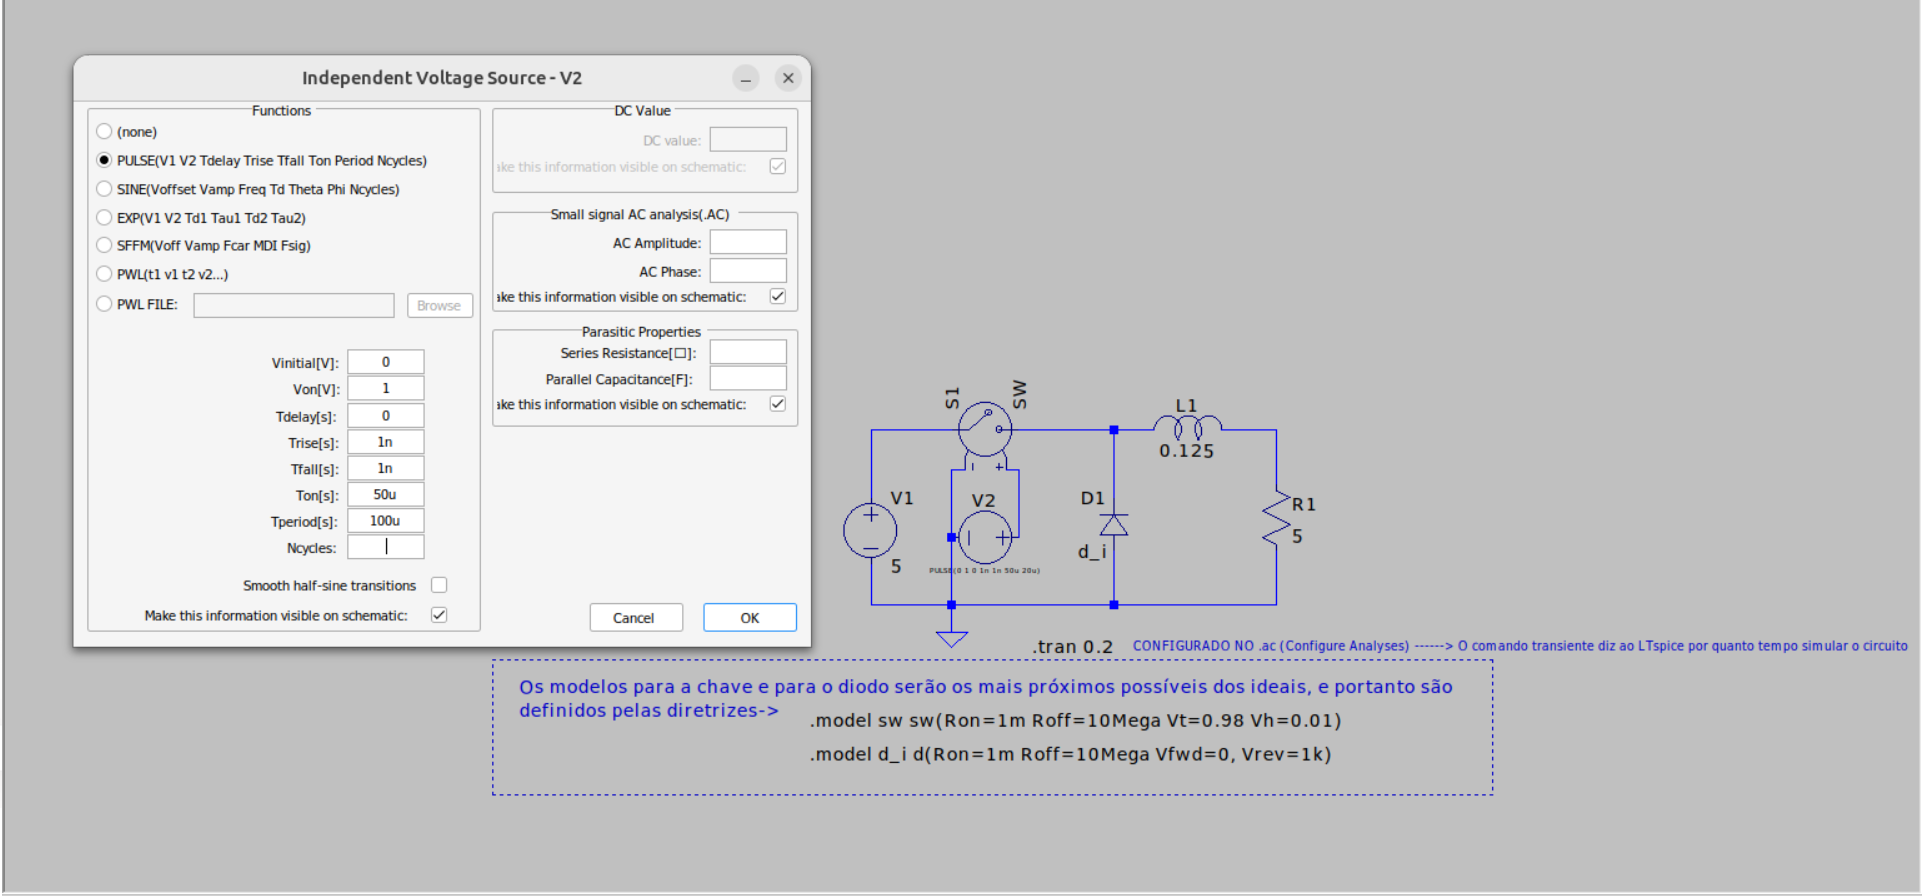
\includegraphics[width=0.6\textwidth]{FIGURAS/circuito_cenario_1.png}
	\caption{Esquemático do Cenário 1 simulado no LTSpice evidenciando o pulso a 10 kHz.}
	\label{fig:sim_cenario1}
\end{figure}

O comportamento dinâmico é elucidado pelas Figuras \ref{fig:trans_1} e \ref{fig:perm_1}. No regime transitório, nota-se a elevação assintótica da tensão acompanhando a magnetização gradual do grande indutor. No regime permanente, o uso da ferramenta de cursores atestou a obtenção do perfil em "dente de serra" previso teoricamente.

\begin{figure}[H]
	\centering
	\begin{minipage}{0.45\textwidth}
		\centering
		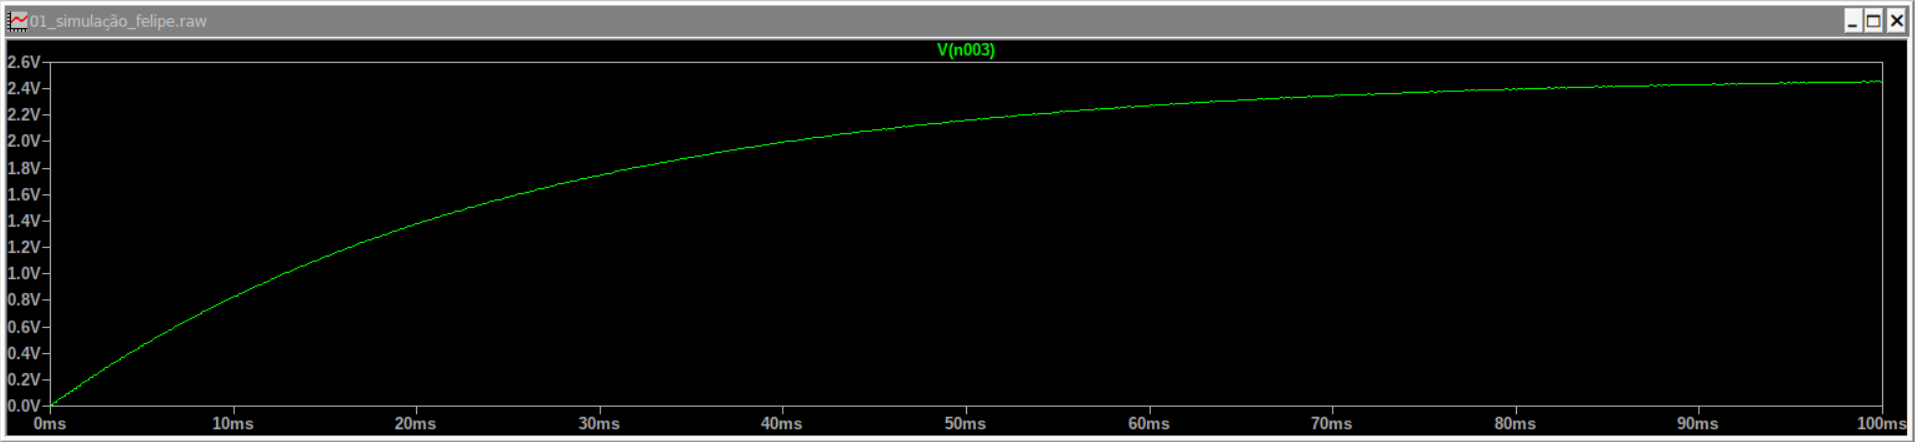
\includegraphics[width=\textwidth]{FIGURAS/transitorio_1.png}
		\caption{Visão ampla do regime transitório inicial (Cenário 1).}
		\label{fig:trans_1}
	\end{minipage}\hfill
	\begin{minipage}{0.45\textwidth}
		\centering
		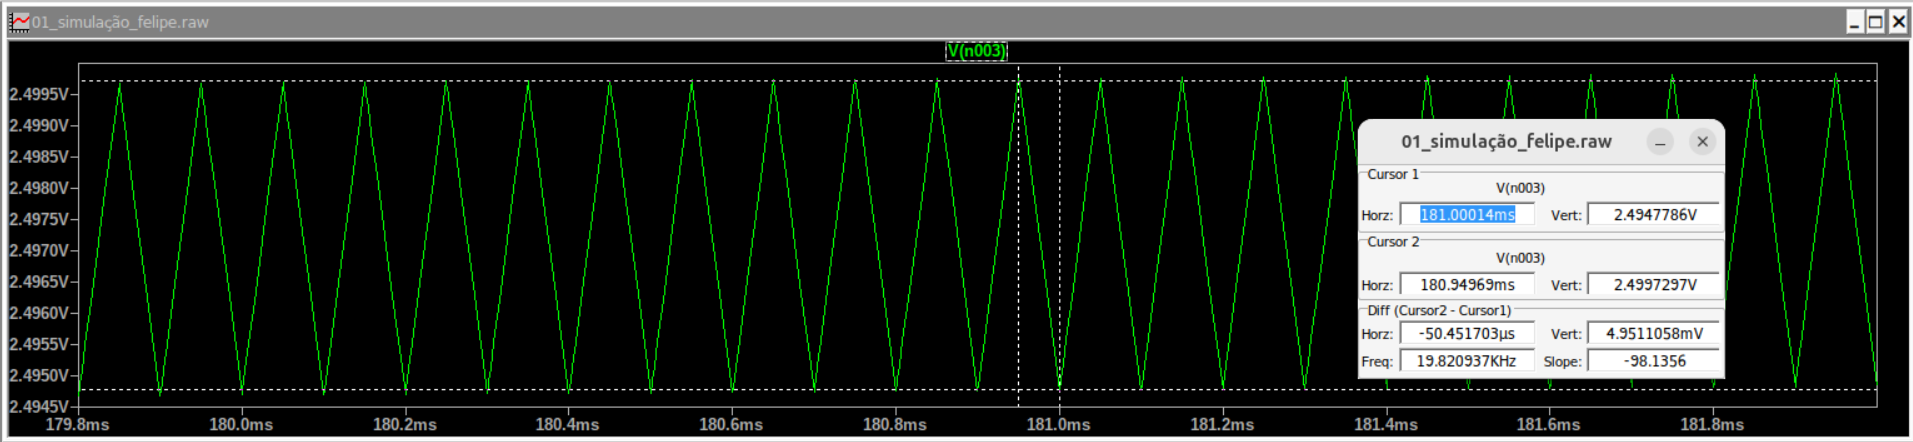
\includegraphics[width=\textwidth]{FIGURAS/permanente_1.png} 
		\caption{Zoom no regime permanente ilustrando a medição da ondulação ($\Delta V$).}
		\label{fig:perm_1}
	\end{minipage}
\end{figure}

\section{Cenário 2: $R = 5\,\Omega$, $f = 50\text{ kHz}$ e $L = 25\text{ mH}$}

Mantendo a resistência de $5\,\Omega$, a elevação da frequência de chaveamento em cinco vezes (para $50\text{ kHz}$) permitiu a redução proporcional da indutância para $25\text{ mH}$, mantendo o projeto estrito ao limite de ondulação admissível.

\begin{figure}[H]
	\centering
	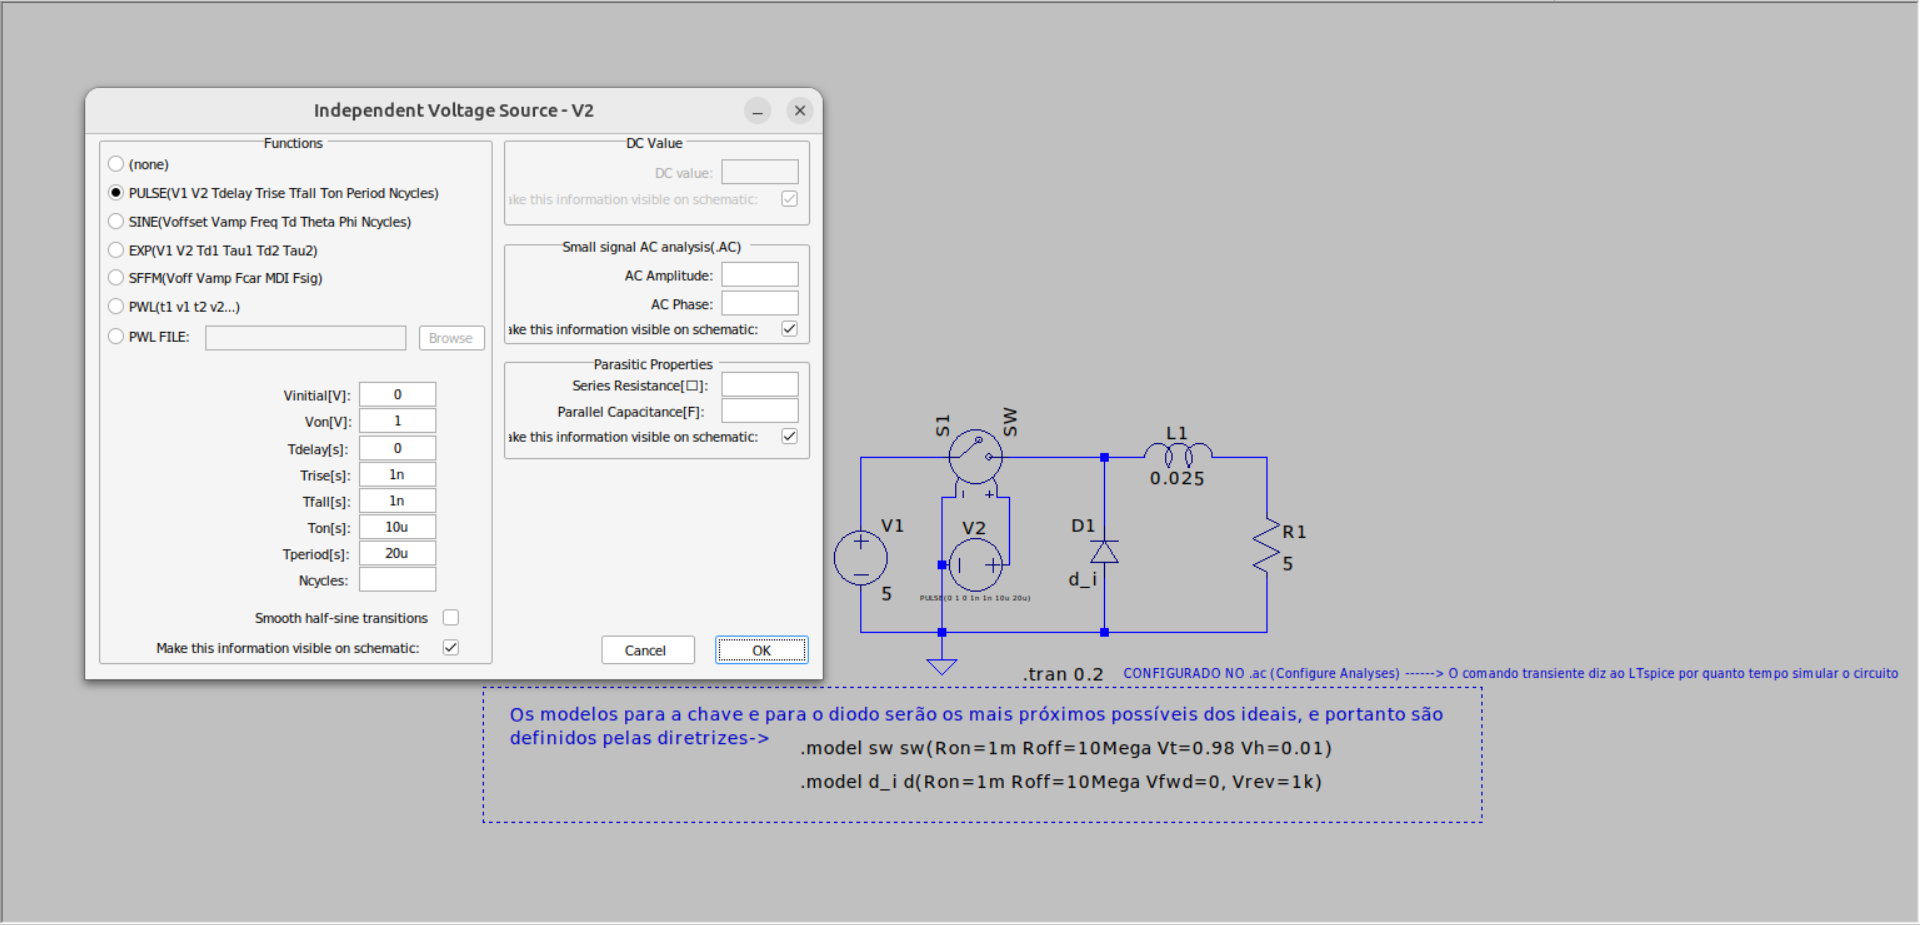
\includegraphics[width=0.6\textwidth]{FIGURAS/circuito_cenario_2.png}
	\caption{Esquemático do Cenário 2 no LTSpice configurado para 50 kHz.}
	\label{fig:sim_cenario2}
\end{figure}

A dinâmica temporal registrada corrobora que a frequência mais alta diminui significativamente a energia transferida por ciclo, mantendo o nível contínuo estável e o \textit{ripple} estritamente confinado dentro da margem imposta.

\begin{figure}[H]
	\centering
	\begin{minipage}{0.45\textwidth}
		\centering
		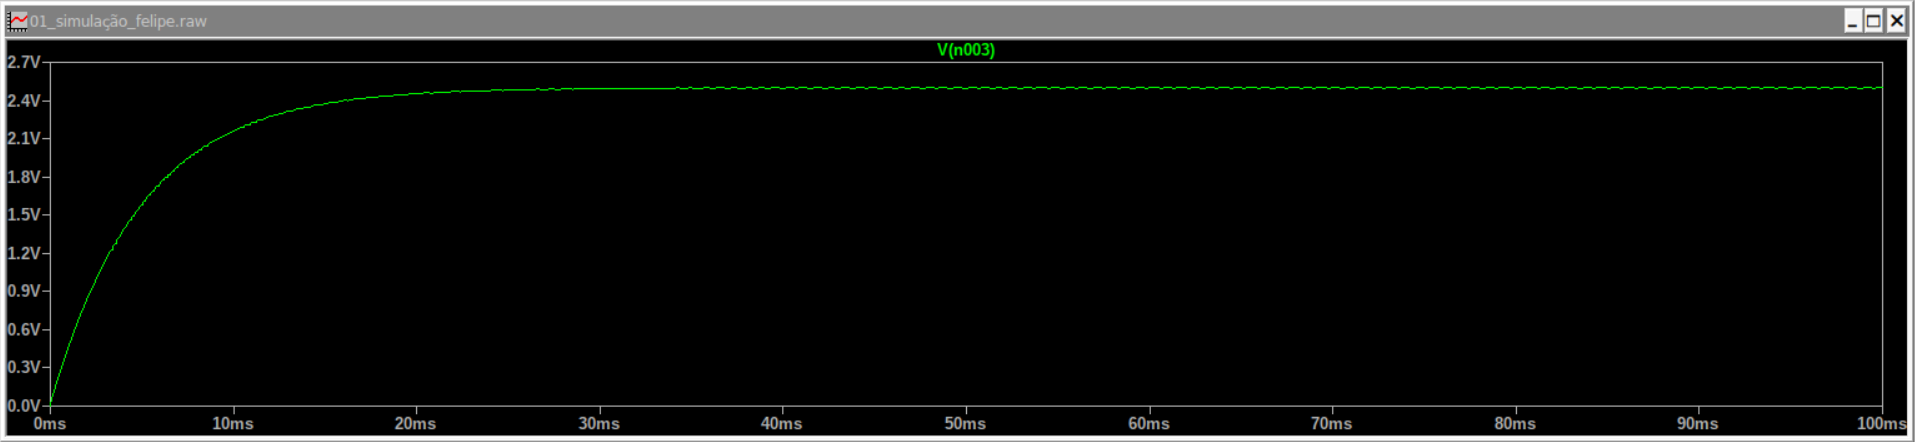
\includegraphics[width=\textwidth]{FIGURAS/transitorio_2.png}
		\caption{Resposta em regime transitório (Cenário 2).}
		\label{fig:trans_2}
	\end{minipage}\hfill
	\begin{minipage}{0.45\textwidth}
		\centering
		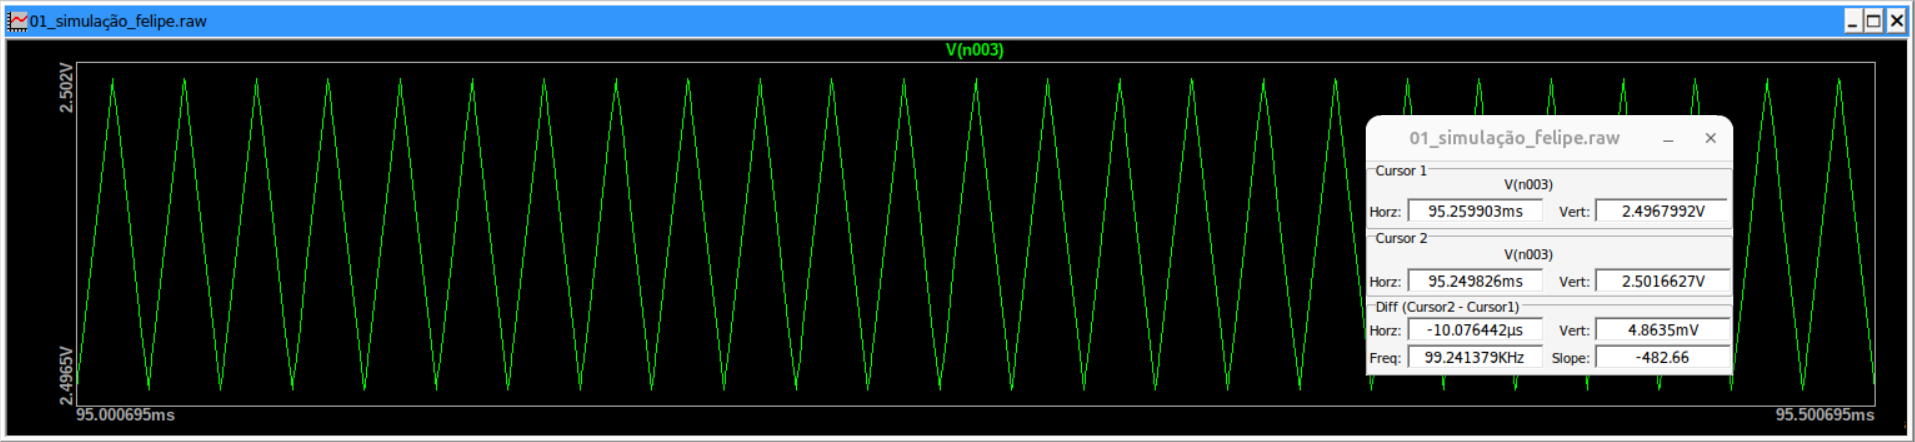
\includegraphics[width=\textwidth]{FIGURAS/permanente_2.png} 
		\caption{Forma de onda estável em regime permanente.}
		\label{fig:perm_2}
	\end{minipage}
\end{figure}

\section{Cenário 3: $R = 1\,\Omega$, $f = 10\text{ kHz}$ e $L = 25\text{ mH}$}

Neste ensaio, a resistência de carga sofreu redução para $1\,\Omega$, o que aumenta a severidade da corrente exigida pela saída do conversor. O pulso de controle retorna para $10\text{ kHz}$, demandando um indutor de $25\text{ mH}$.

\begin{figure}[H]
	\centering
	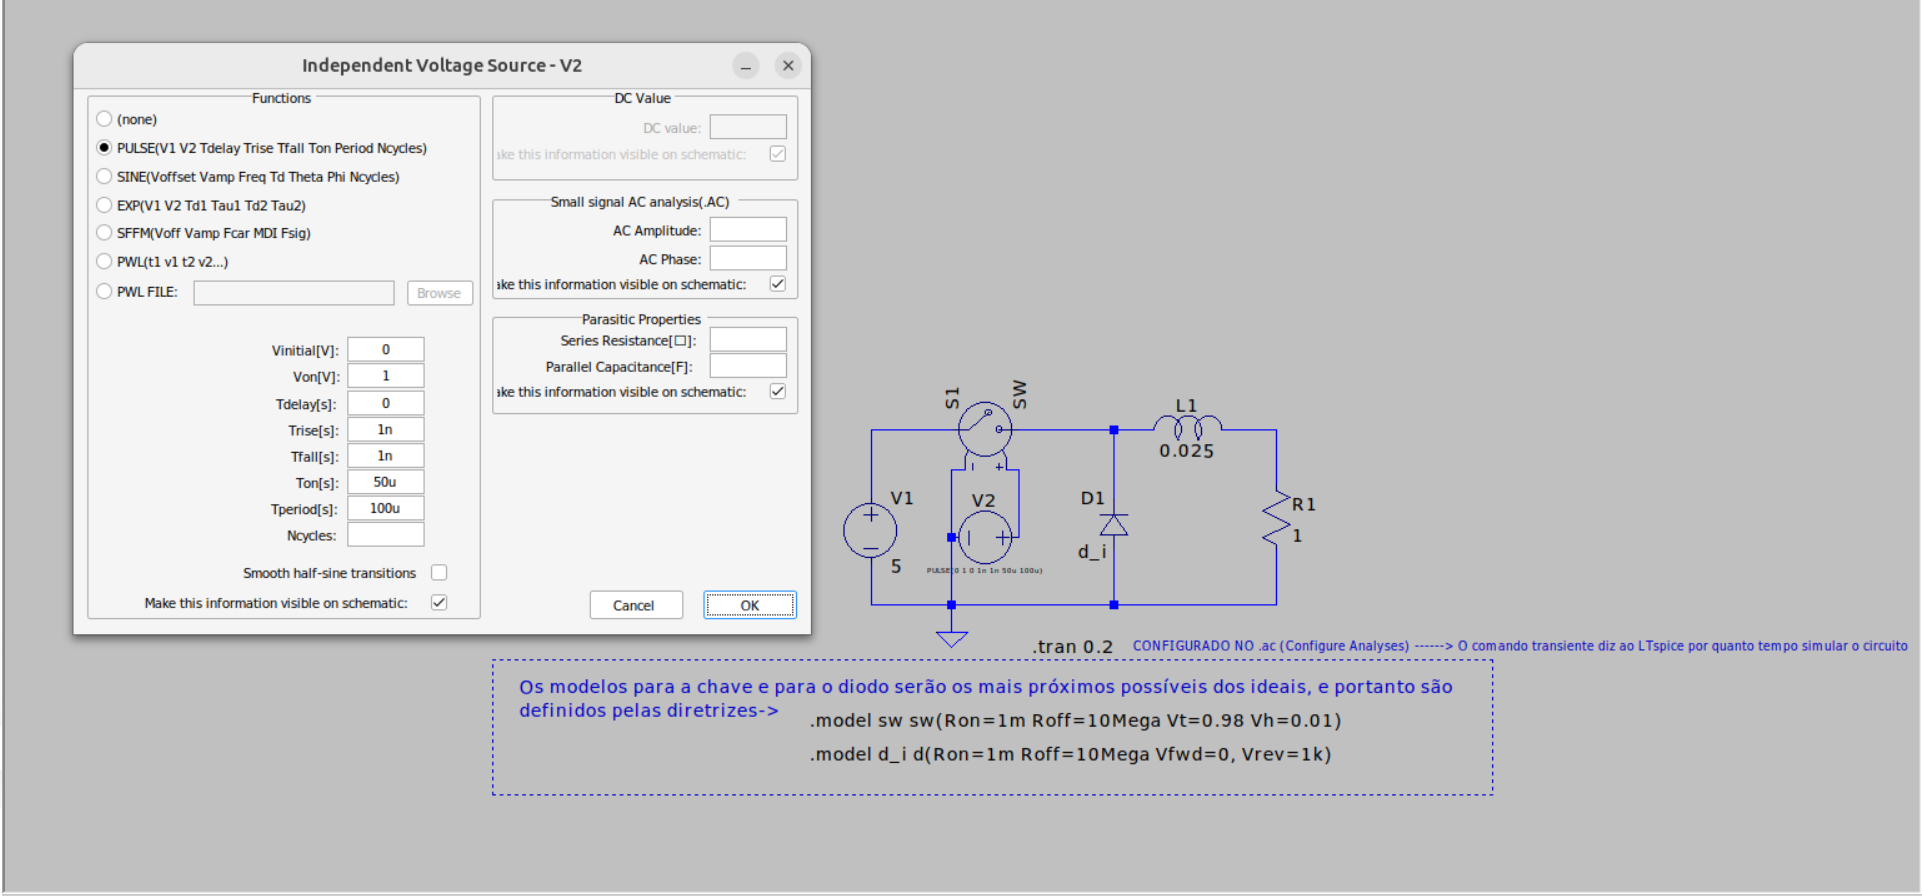
\includegraphics[width=0.6\textwidth]{FIGURAS/circuito_cenario_3.png}
	\caption{Esquemático do Cenário 3 evidenciando a alteração da carga e o pulso de controle.}
	\label{fig:sim_cenario3}
\end{figure}

Como a constante de tempo do sistema ($\tau = L/R$) alterou-se, o tempo de acomodação para atingir o regime permanente reduziu drasticamente frente aos cenários anteriores, observando-se uma subida vertiginosa na curva do regime transitório.

\begin{figure}[H]
	\centering
	\begin{minipage}{0.45\textwidth}
		\centering
		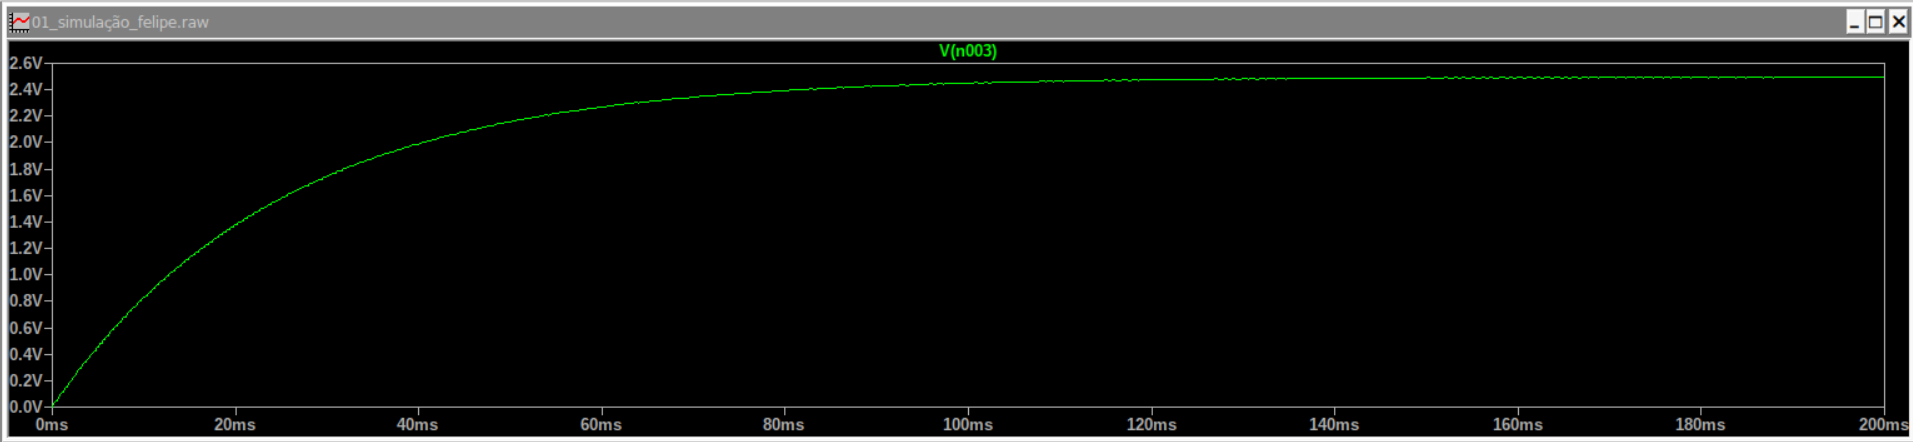
\includegraphics[width=\textwidth]{FIGURAS/transitorio_3.png}
		\caption{Carregamento acelerado do indutor no regime transitório (Cenário 3).}
		\label{fig:trans_3}
	\end{minipage}\hfill
	\begin{minipage}{0.45\textwidth}
		\centering
		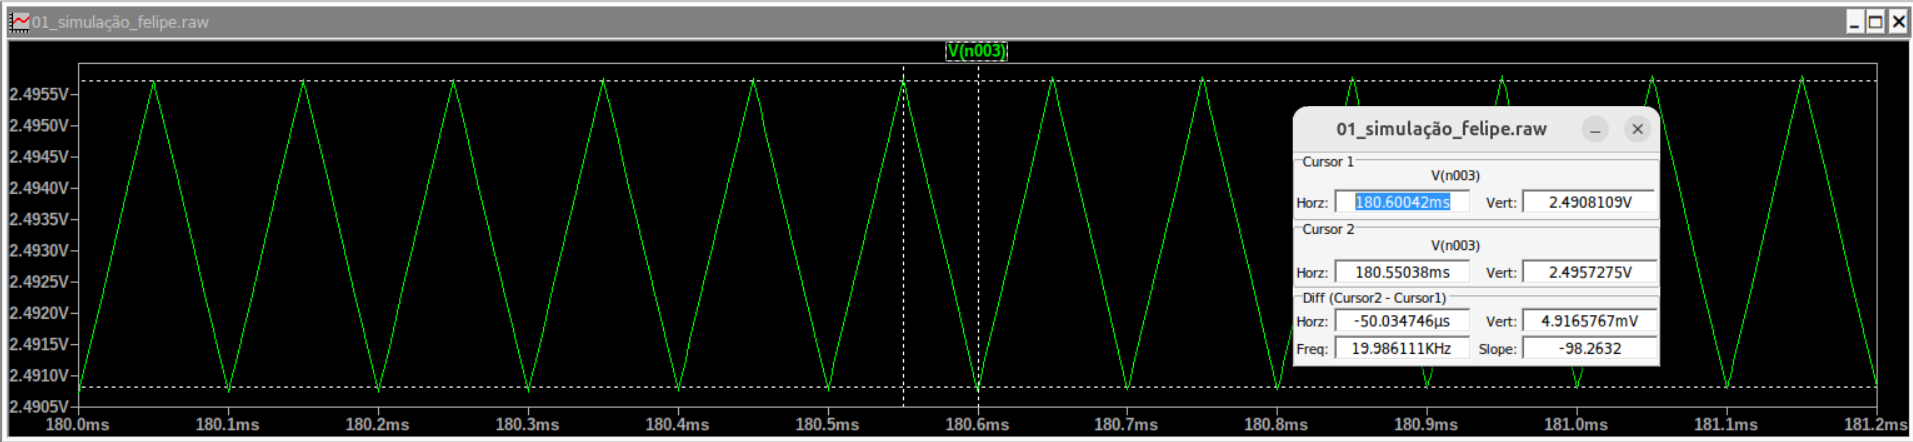
\includegraphics[width=\textwidth]{FIGURAS/permanente_3.png} 
		\caption{Dentes de serra na extração do pico e vale de tensão.}
		\label{fig:perm_3}
	\end{minipage}
\end{figure}

\section{Cenário 4: $R = 1\,\Omega$, $f = 50\text{ kHz}$ e $L = 5\text{ mH}$}

O quarto e último cenário agrupa as condições críticas de alta demanda de corrente ($1\,\Omega$) e alta comutação ($50\text{ kHz}$). Esta combinação projeta o menor elemento magnético da prática, um indutor de apenas $5\text{ mH}$.

\begin{figure}[H]
	\centering
	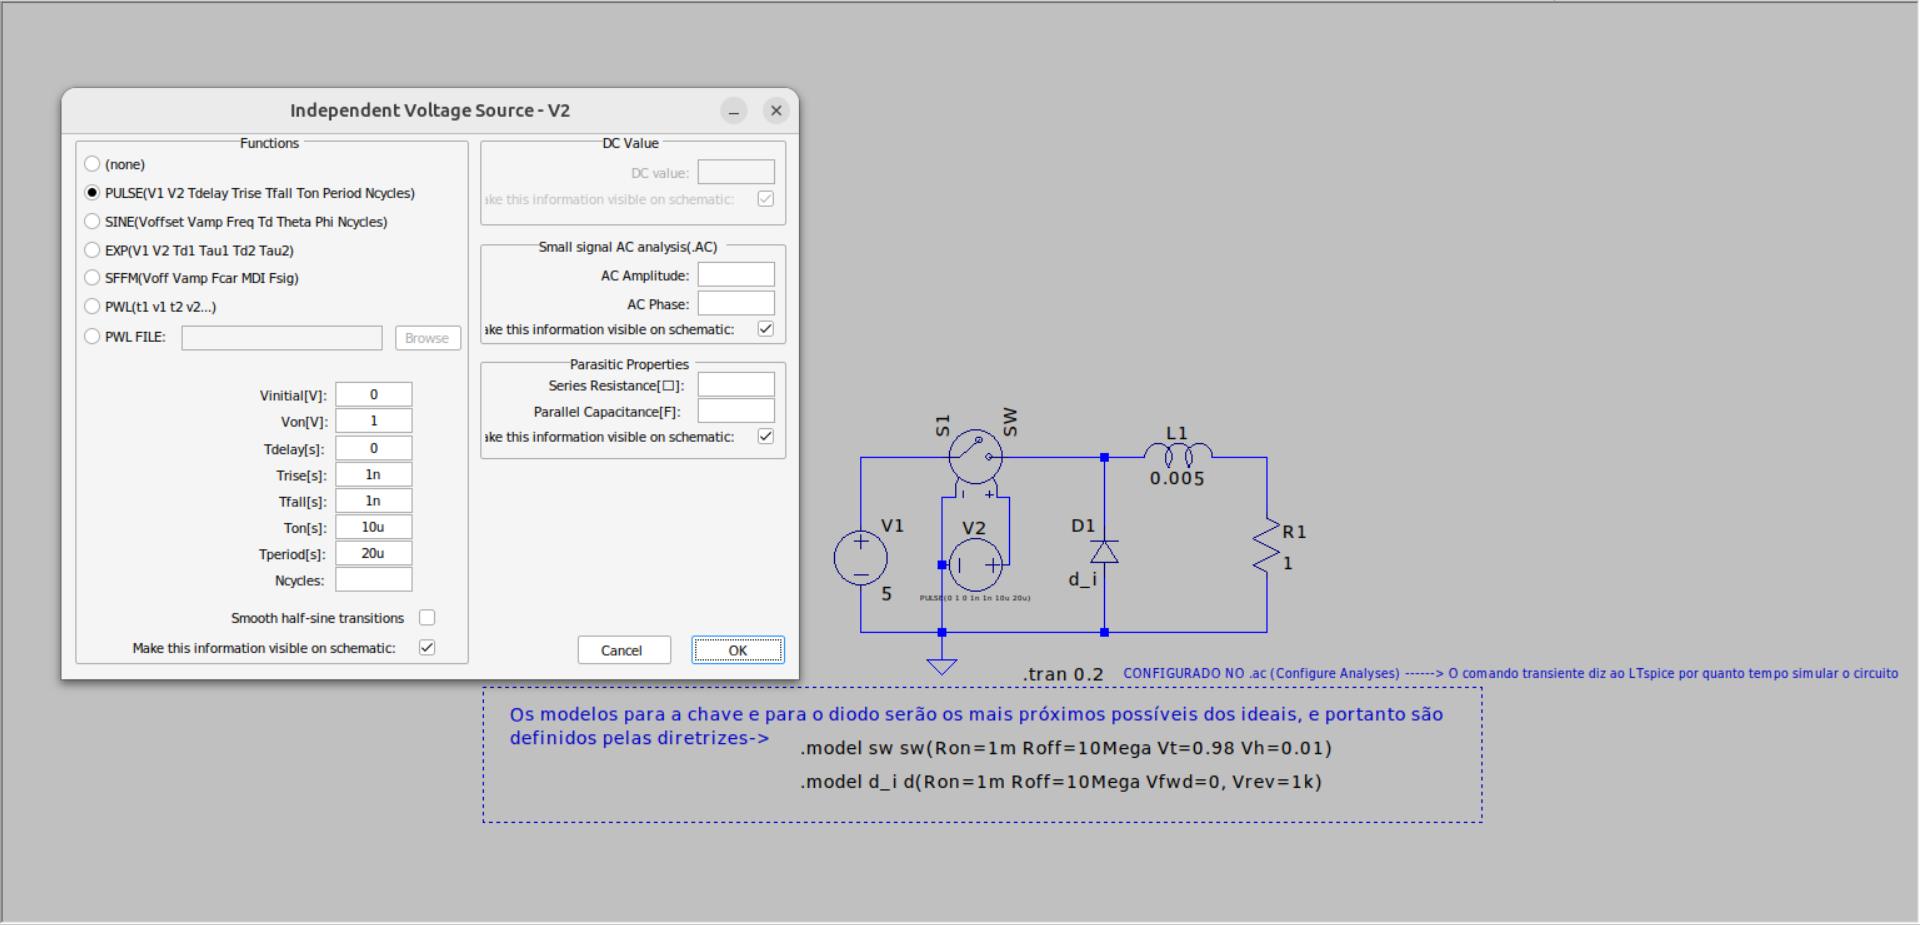
\includegraphics[width=0.6\textwidth]{FIGURAS/circuito_cenario_4.png}
	\caption{Esquemático final (Cenário 4) parametrizado no LTSpice.}
	\label{fig:sim_cenario4}
\end{figure}

A simulação transiente deste arranjo prova que componentes magnéticos ultracompactos podem ser aplicados em fontes chaveadas contanto que a velocidade do chaveamento seja suficiente para não saturar o núcleo. O \textit{ripple} observado manteve-se ínfimo.

\begin{figure}[H]
	\centering
	\begin{minipage}{0.45\textwidth}
		\centering
		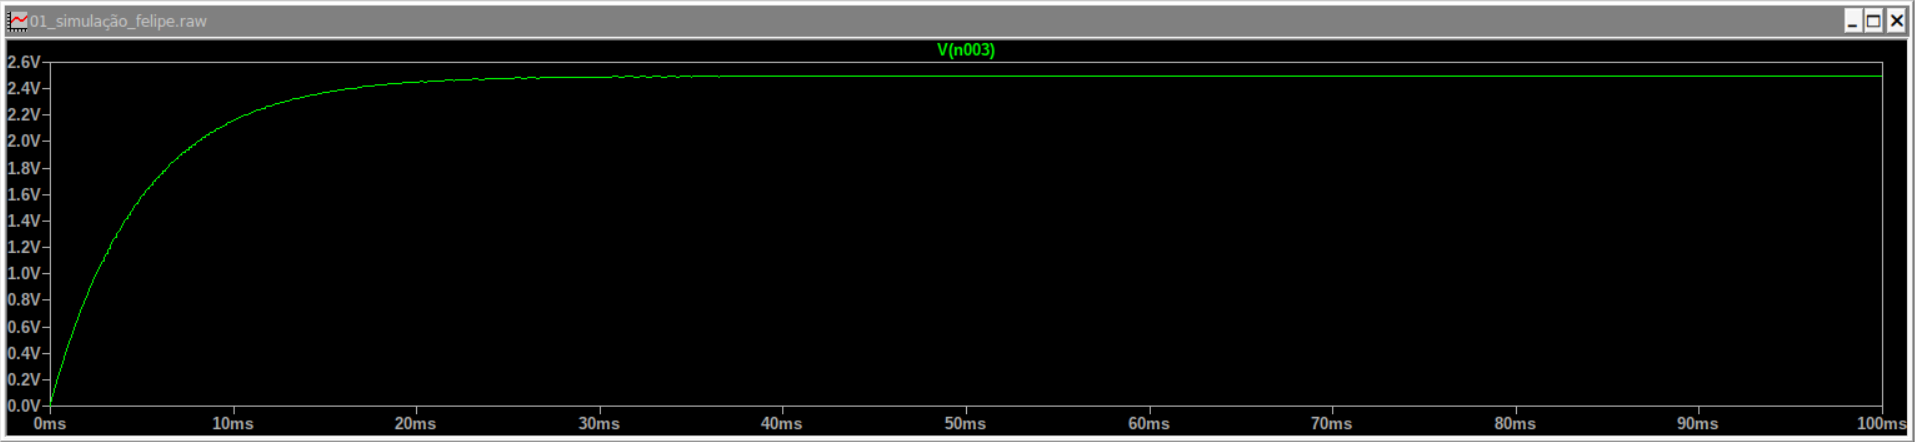
\includegraphics[width=\textwidth]{FIGURAS/transitorio_4.png}
		\caption{Regime transitório para carga pesada em alta comutação (Cenário 4).}
		\label{fig:trans_4}
	\end{minipage}\hfill
	\begin{minipage}{0.45\textwidth}
		\centering
		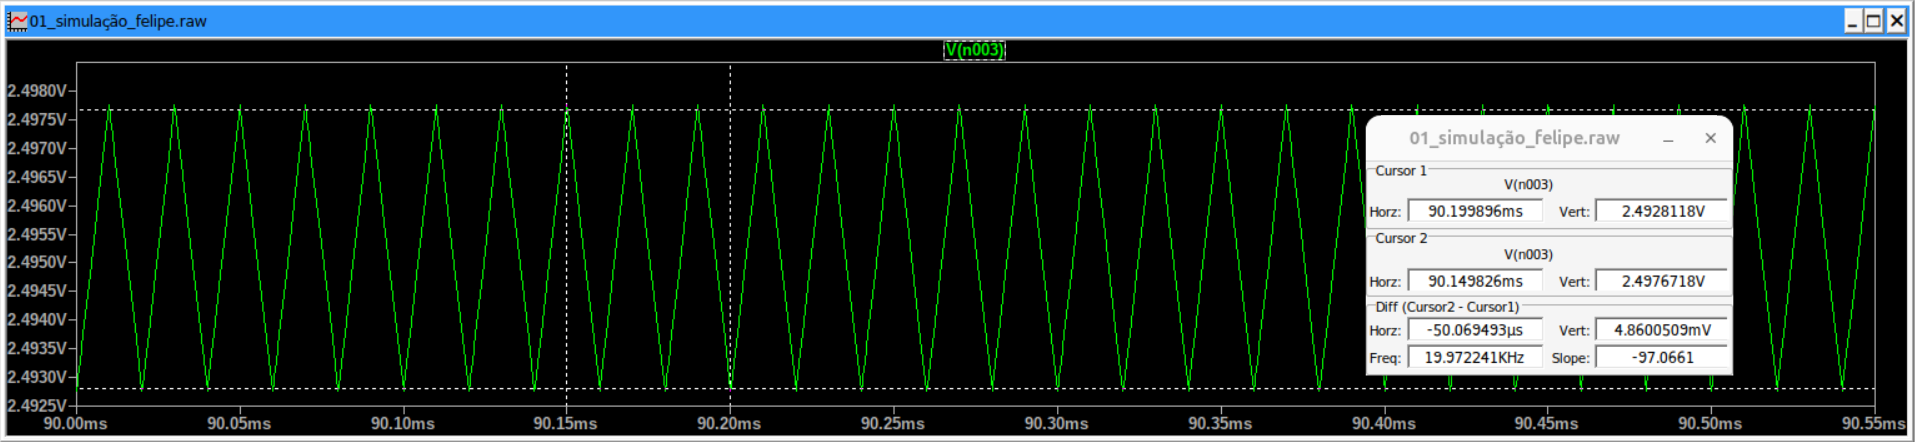
\includegraphics[width=\textwidth]{FIGURAS/permanente_4.png} 
		\caption{Regime permanente validando o comportamento global do filtro.}
		\label{fig:perm_4}
	\end{minipage}
\end{figure}